\subsection{Refinement of the Six Bar Method}
The method as stated above suffers from a fundamental asymmetry in the
way the counters are used in the calculations (as shown in the table
below): The inner two counters are each involved in four of the $T_k$,
whereas the next outer two are only necessary for three each and the
outer most are only used in two of the $T_k$; this causes some
counters to have a stronger influence on the computed counter
resolutions than others.  In practice this results in large
fluctuations in the computed counter resolutions, but can be helped
with a slight modification to the method.\\

\begin{tabular}[c]{c || c || c}
  Counter & \# of Dependent $T_k$ & Dependent Combinations\\ \hline
  1 & 2 & (1,2,3), (1,3,5)\\
  2 & 3 & (1,2,3), (2,3,4),(2,4,6)\\
  3 & 4 & (1,2,3), (2,3,4), (3,4,5), (1,3,5)\\
  4 & 4 & (2,3,4), (3,4,5), (4,5,6), (2,4,6)\\
  5 & 3 & (3,4,5), (4,5,6), (1,3,5)\\
  6 & 2 & (4,5,6), (2,4,6)\\
\end{tabular}\\

To remedy this, two consecutive 6-bar measurements are run instead of
one, with the second measurement having the counters stacked in a
different order (known as the \textit{complementary ordering}).  The
order was selected to make the number of equations containing each
counter resolution the same, and is described by the permutation, from
top to bottom, (3,2,1,6,5,4).

\begin{figure}[H]
  \centering
  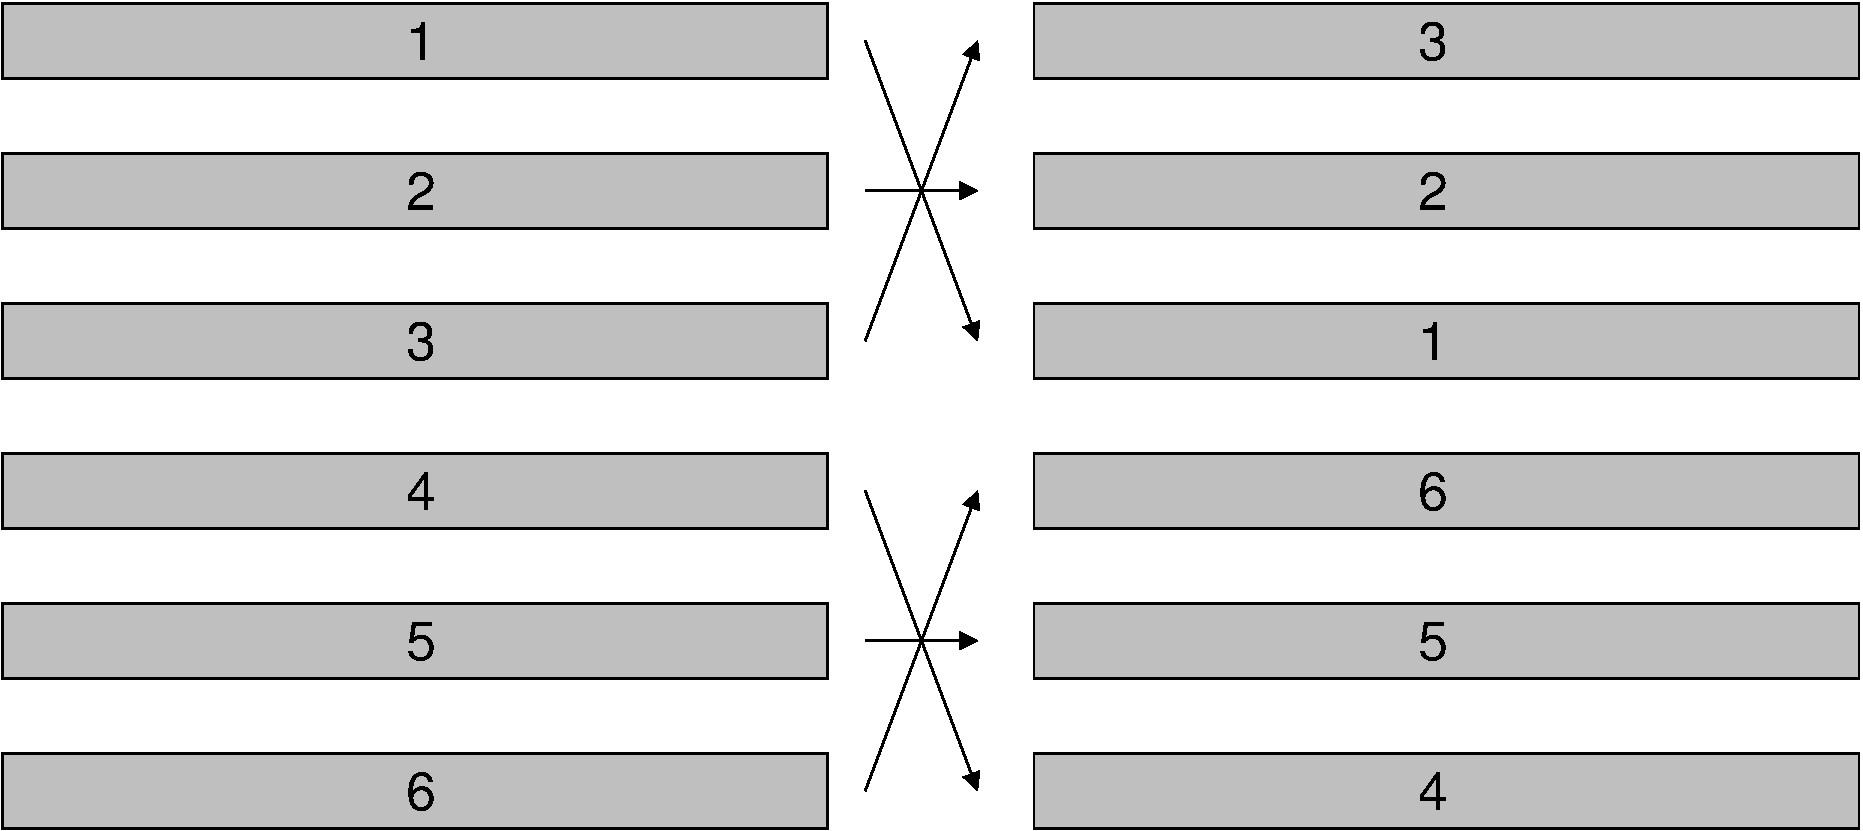
\includegraphics[width=15cm]{gary/fig_gary_six_bar_refinement/complementary.pdf}
  \caption{Rearrangement of the six counters for the complementary
    measurement.}
  \label{complementary}
\end{figure}

The additional three bar observables are

\begin{equation}
  T_{(3,2,1)} = (t_3 + t_1)/2 - t_2,
\end{equation}
\begin{equation}
  T_{(2,1,6)} = (t_2 + t_6)/2 - t_1,
\end{equation}
\begin{equation}
  T_{(1,6,5)} = (t_1 + t_5)/2 - t_6,
\end{equation}
\begin{equation}
  T_{(6,5,4)} = (t_6 + t_4)/2 - t_5,
\end{equation}
\begin{equation}
  T_{(3,1,5)} = (t_3 + t_5)/2 - t_1,
\end{equation}
\begin{equation}
  T_{(2,6,4)} = (t_2 + t_4)/2 - t_6,
\end{equation}

leading to the following over-constrained system of equations for the
individual counter resolutions,

\begin{equation}
  \begin{cases}
    \sigma_{T_{(1,2,3)}}^2 = (\sigma_1^2 + \sigma_3^2)/4 + \sigma_2^2\\
    \sigma_{T_{(2,3,4)}}^2 = (\sigma_2^2 + \sigma_4^2)/4 + \sigma_3^2\\
    \sigma_{T_{(3,4,5)}}^2 = (\sigma_3^2 + \sigma_5^2)/4 + \sigma_4^2\\
    \sigma_{T_{(4,5,6)}}^2 = (\sigma_4^2 + \sigma_6^2)/4 + \sigma_5^2\\
    \sigma_{T_{(1,3,5)}}^2 = (\sigma_1^2 + \sigma_5^2)/4 + \sigma_3^2\\
    \sigma_{T_{(2,4,6)}}^2 = (\sigma_2^2 + \sigma_6^2)/4 + \sigma_4^2\\
    \sigma_{T_{(3,2,1)}}^2 = (\sigma_3^2 + \sigma_1^2)/4 - \sigma_2^2\\
    \sigma_{T_{(2,1,6)}}^2 = (\sigma_2^2 + \sigma_6^2)/4 - \sigma_1^2\\
    \sigma_{T_{(1,6,5)}}^2 = (\sigma_1^2 + \sigma_5^2)/4 - \sigma_6^2\\
    \sigma_{T_{(6,5,4)}}^2 = (\sigma_6^2 + \sigma_4^2)/4 - \sigma_5^2\\
    \sigma_{T_{(3,1,5)}}^2 = (\sigma_3^2 + \sigma_5^2)/4 - \sigma_1^2\\
    \sigma_{T_{(2,6,4)}}^2 = (\sigma_2^2 + \sigma_4^2)/4 - \sigma_6^2
  \end{cases}
\end{equation}

and in matrix form,

\begin{equation}
  \left[\begin{array}{c}
      \sigma_{T_{(1,2,3)}}^2 \\
      \sigma_{T_{(2,3,4)}}^2 \\
      \sigma_{T_{(3,4,5)}}^2 \\
      \sigma_{T_{(4,5,6)}}^2 \\
      \sigma_{T_{(1,3,5)}}^2 \\
      \sigma_{T_{(2,4,6)}}^2 \\

      \sigma_{T_{(3,2,1)}}^2 \\
      \sigma_{T_{(2,1,6)}}^2 \\
      \sigma_{T_{(1,6,5)}}^2 \\
      \sigma_{T_{(6,5,4)}}^2 \\
      \sigma_{T_{(3,1,5)}}^2 \\
      \sigma_{T_{(2,6,4)}}^2 \\
    \end{array}
    \right]
  = \left[ \begin{array}{cccccc}
      \frac{1}{4} & 1 & \frac{1}{4} & 0 & 0 & 0 \\
      0 & \frac{1}{4} & 1 & \frac{1}{4} & 0 & 0 \\
      0 & 0 & \frac{1}{4} & 1 & \frac{1}{4} & 0 \\
      0 & 0 & 0 & \frac{1}{4} & 1 & \frac{1}{4} \\
      \frac{1}{4} & 0 & 1 & 0 & \frac{1}{4} & 0 \\
      0 & \frac{1}{4} & 0 & 1 & 0 & \frac{1}{4}\\

      \frac{1}{4} & 1 & \frac{1}{4} & 0 & 0 & 0 \\
      1 & \frac{1}{4} & 0 & 0 & 0 & \frac{1}{4} \\
      \frac{1}{4} & 0 & 0 & 0 & \frac{1}{4} & 1 \\
      0 & 0 & 0 & \frac{1}{4} & 1 & \frac{1}{4} \\
      1 & 0 & \frac{1}{4} & 0 & \frac{1}{4} & 0 \\
      0 & \frac{1}{4} & 0 & \frac{1}{4} & 0 & 1 \\
    \end{array}
    \right]
  \left[
    \begin{array}{c}
      \sigma_1^2 \\
      \sigma_2^2 \\
      \sigma_3^2 \\
      \sigma_4^2 \\
      \sigma_5^2 \\
      \sigma_6^2 \\
    \end{array}
    \right],
\end{equation}

or just

\begin{equation}
  \vec{T} = \hat{A} \vec{\sigma}.
\end{equation}

%I need to add some pictures showing the results of using the combined
%measurements vs. just the original six bar method.
In the combined over-constrained system of equations, each counter
resolution occurs in six equations.  This modification makes the
method noticeably more stable when computing the individual counter
resolutions.  As the new system of equations is over-constrained, the
best estimator for the solution to the system is given by the method
of linear least-squares.  Linear least-squares consists of solving the
following equation for \(\vec{\sigma}\):

\begin{equation}
  (\hat{A}^T \hat{A}) \vec{\sigma} = \hat{A}^T \vec{T}.
\end{equation}

%% Need to add figure showing how normal+complementary is more stable
%% than just normal or complementary ordering (independent of
%% statistics since normal+complementary has more statistics than
%% either normal or complementary alone).
